\usepackage{ifthen}

% Define an agenda item
%
% Arguments:
% 1: Identifier of the agenda item, should be all lower-case
% 2: Type of the agenda item: lecture or lab
% 3: English title of the agenda item
% 4: English full description of the agenda item
% 5: French title of the agenda item
% 6: French full description of the agenda item
\newcommand\defagendaitem[6]{
  \ifthenelse{\equal{\agendalanguage}{french}}{
    \expandafter\def\csname #1@#2@title\endcsname {#5}
    \expandafter\def\csname #1@#2@contents\endcsname {#6}
  }{
    \expandafter\def\csname #1@#2@title\endcsname {#3}
    \expandafter\def\csname #1@#2@contents\endcsname {#4}
  }
}

% Show/render an agenda item
%
% Arguments:
% 1: Identifier of the agenda item, as defined by \defagendaitem
% 2: Type of the agenda item: lecture or lab
\newcommand\showagendaitem[2]{%
  \ifthenelse{\boolean{hlineneeded}}{\\\hline}{\setboolean{hlineneeded}{true}}%
    \ifthenelse{\equal{\agendalanguage}{french}}{%
      \ifthenelse{\equal{#2}{lecture}}%
      {Cours &}%
      {%
        \ifthenelse{\equal{#2}{lab}}{%
          \ifthenelse{\equal{\trainingtype}{online}}{Démo &}{TP &}%
        }%
        {}%
      }%
    }{%
      \ifthenelse{\equal{#2}{lecture}}%
      {Lecture &}%
      {%
        \ifthenelse{\equal{#2}{lab}}{%
          \ifthenelse{\equal{\trainingtype}{online}}{Demo &}{Lab &}%
        }%
        {}%
      }%
    }%
    \csname #1@#2@title\endcsname &%
    \vspace{-12pt}%
    \csname #1@#2@contents\endcsname%
}%

% Define a board
%
% Arguments:
% 1: Identifier for the board, must be all lower-case
% 2: English title
% 3: English full description
% 4: French title
% 5: French full description
% 6: Board picture
\newcommand\defboard[6]{
  \ifthenelse{\equal{\agendalanguage}{french}}{
    \expandafter\def\csname #1@title\endcsname {#4}
    \expandafter\def\csname #1@contents\endcsname {#5}
  }{
    \expandafter\def\csname #1@title\endcsname {#2}
    \expandafter\def\csname #1@contents\endcsname {#3}
  }
  \expandafter\def\csname #1@image\endcsname {#6}
}

% Show/render a board
%
% Arguments:
% 1: Identifier of the board, as defined by \defboard
\newcommand\showboarditem[1]{
  \begin{tabularx}{\textwidth}{p{7cm}p{11cm}}
    \arrayrulecolor{blorange}
    \hline
    \multicolumn{1}{l}{\textbf{\textcolor{blorange}{\large \csname #1@title\endcsname}}} & \\
    \hline
    \arrayrulecolor{gray}
    \csname #1@contents\endcsname &
    \csname #1@image\endcsname \\
  \end{tabularx}
}

% Start an agenda by finding
% out if it is a morning or an
% afternoon if the training
% takes place on site
%
% Arguments:
% 1: Number of the half-day
\newcommand\showagendaday[1]{%
  \arrayrulecolor{blorange}%
  \\\hline%
  \multicolumn{3}{l}{%
    \textbf{\textcolor{blorange}{\large%
      \ifthenelse{\equal{\trainingtype}{online}}{%
        \showonlineagendaday{#1}%
      }{%
        \pgfmathparse{int(mod(#1, 2))}%
        \ifnum\pgfmathresult=1%
          \pgfmathparse{int((#1 + 1) / 2)}%
          \showonsiteagendaday{\pgfmathresult}{morning}%
        \else%
          \pgfmathparse{int(#1 / 2)}%
          \showonsiteagendaday{\pgfmathresult}{afternoon}%
        \fi%
      }%
    }}%
  } \\%
  \hline%
  \setboolean{hlineneeded}{false}%
  \arrayrulecolor{gray}%
}%

% Start an online agenda half-day
%
% Arguments:
% 1: Number of the half-day
\newcommand\showonlineagendaday[1]{%
  \ifthenelse{\equal{\agendalanguage}{french}}{%
    Demi-journée #1%
  }{%
    Half day #1%
  }%
}%

% Start an on-site agenda half-day
%
% Arguments:
% 1: Number of the day
% 2: "morning" or "afternoon"
\newcommand\showonsiteagendaday[2]{%
  \ifthenelse{\equal{\agendalanguage}{french}}{%
    \ifthenelse{\equal{#2}{morning}}{%
      Jour #1 - Matin%
    }{%
      Jour #1 - Après-midi%
    }%
  }{%
    \ifthenelse{\equal{#2}{morning}}{%
      Day #1 - Morning%
    }{%
      Day #1 - Afternoon%
    }%
  }%
}%

\defboard
{stm32mp1}
{STM32MP1 Discovery Kit}
{
  One of these Discovery Kits from STMicroelectronics: {\bf
  STM32MP157A-DK1}, {\bf STM32MP157D-DK1}, {\bf STM32MP157C-DK2} or
  {\bf STM32MP157F-DK2}
  \begin{itemize}
  \item STM32MP157, dual Cortex-A7 processor from STMicroelectronics
  \item USB powered
  \item 512 MB DDR3L RAM
  \item Gigabit Ethernet port
  \item 4 USB 2.0 host ports
  \item 1 USB-C OTG port
  \item 1 Micro SD slot
  \item On-board ST-LINK/V2-1 debugger
  \item Arduino compatible headers
  \item Audio codec, buttons, LEDs
  \item LCD touchscreen (DK2 kits only)
  \vspace{-0.7cm}
  \end{itemize}
}
{Plateforme STM32MP1}
{
  Une de ces cartes de STMicroelectronics : {\bf
  STM32MP157A-DK1}, {\bf STM32MP157D-DK1}, {\bf STM32MP157C-DK2} ou
  {\bf STM32MP157F-DK2}
  \begin{itemize}
  \item Processeur STM32MP157, double Cortex-A7, de STMicroelectronics
  \item Alimentée par USB
  \item 512 Mo DDR3L RAM
  \item Port Gigabit Ethernet port
  \item 4 ports hôte USB 2.0
  \item 1 port USB-C OTG
  \item 1 connecteur Micro SD
  \item Debugger ST-LINK/V2-1 sur la carte
  \item Connecteurs compatibles Arduino Uno v3
  \item Codec audio
  \item Divers : boutons, LEDs
  \item Écran LCD tactile (uniquement sur cartes DK2)
  \vspace{-0.7cm}
  \end{itemize}
}
{
  \begin{center}
    \includegraphics[width=5cm]{../slides/discovery-board-dk1/discovery-board-dk1.png}
  \end{center}
}

\defagendaitem
{qna}
{misc}
{Questions and Answers}
{
  \begin{itemize}
  \item Questions and answers with the audience about the course topics
  \item Extra presentations if time is left, according what most
        participants are interested in.
  \end{itemize}
}
{Questions / réponses}
{
  \begin{itemize}
  \item Questions et réponses avec les participants à propos des sujets abordés.
  \item Présentations supplémentaires s'il reste du temps, en fonction des demandes
        de la majorité des participants.
  \end{itemize}
}


\defboard
{beagleboneblack}
{BeagleBone Black}
{
  {\bf BeagleBone Black} or {\bf BeagleBone Black Wireless} board
  \begin{itemize}
  \item An ARM AM335x (single Cortex-A8) processor from Texas
    Instruments
  \item USB powered
  \item 512 MB of RAM
  \item 2 or 4 GB of on-board eMMC storage
  \item USB host and device
  \item HDMI output
  \item 2 x 46 pins headers, to access UARTs, SPI buses, I2C buses
    and more.
  \item Ethernet or WiFi
  \end{itemize}
  \vspace{-0.7cm}
}
{BeagleBone Black}
{
  Carte {\bf BeagleBone Black} ou {\bf BeagleBone Black Wireless}
  \begin{itemize}
  \item Un processeur ARM AM335x de Texas Instruments (à base de
    Cortex-A8), avec accélération 3D, etc.
  \item 512 Mo de RAM
  \item 2 ou 4 Go de stockage eMMC
  \item USB hôte et device
  \item Sortie HDMI
  \item Connecteurs à 2 x 46 broches, pour accéder aux UARTs, aux bus
    SPI, aux bus I2C, et à d'autres entrées/sorties du processeur.
  \item Ethernet ou WiFi
  \vspace{-0.7cm}
  \end{itemize}
}
{
  \begin{center}
    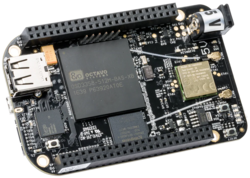
\includegraphics[width=5cm]{../slides/beagleboneblack-board/beagleboneblack_sd.png}
  \end{center}
}

\defboard
{beagleplay}
{BeaglePlay}
{
  {\bf BeaglePlay} board
  \begin{itemize}
    \item Texas Instruments AM625x (4xARM Cortex-A53 CPU)
    \item SoC with 3D acceleration, integrated MCU and many other peripherals.
    \item 2 GB of RAM
    \item 16 GB of on-board eMMC storage
    \item USB host and USB device, microSD, HDMI
    \item 2.4 and 5 GHz WiFi, Bluetooth and also Ethernet
    \item 1 MicroBus Header (SPI, I2C, UART, ...), OLDI and CSI connector.
  \vspace{-0.7cm}
  \end{itemize}
}
{BeaglePlay}
{
  Carte {\bf BeaglePlay}
  \begin{itemize}
    \item SoC Texas Instruments AM625x (CPU 4xARM Cortex-A53)
    \item SoC avec accélération 3D, MCU intégré et de nombreux autres périphériques.
    \item 2 GB de RAM
    \item 16 Go de stockage eMMC
    \item USB hôte et device, microSD, HDMI
    \item WiFi 2.4 and 5 GHz, Bluetooth et aussi Ethernet
    \item 1 Header MicroBus (SPI, I2C, UART, ...), connecteurs OLDI et CSI.
  \vspace{-0.7cm}
  \end{itemize}
}
{
  \begin{center}
    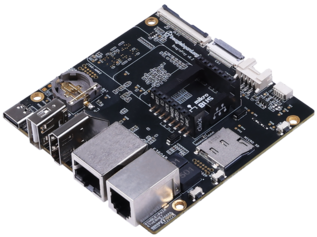
\includegraphics[width=5cm]{../slides/beagleplay-board/beagleplay_sd.png}
  \end{center}
}

\defboard
{espressobin}
{Hardware platform for practical labs}
{
  {\bf Globalscale EspressoBin} board
  \begin{itemize}
  \item Dual Cortex A53 Marvell Armada 3720 SoC
  \item Onboard switch with 2x 1Gbps interfaces
  \item Extra 1Gbps interface
  \item 1GB RAM
  \item 1x SATA interface
  \item 1x USB 3.0 interface
  \end{itemize}
}
{Plateforme matérielle pour les travaux pratiques}
{
  Carte {\bf Globalscale EspressoBin}
  \begin{itemize}
  \item SoC Marvell Armada 3720 SoC (CPU 2xARM Cortex A53)
  \item Switch Ethernet avec 2 interfaces Gigabit
  \item Interface Gigabit Ethernet additionnelle
  \item 1GB de RAM
  \item 1x interface SATA
  \item 1x interface USB 3.0
  \end{itemize}
}
{
  \begin{center}
    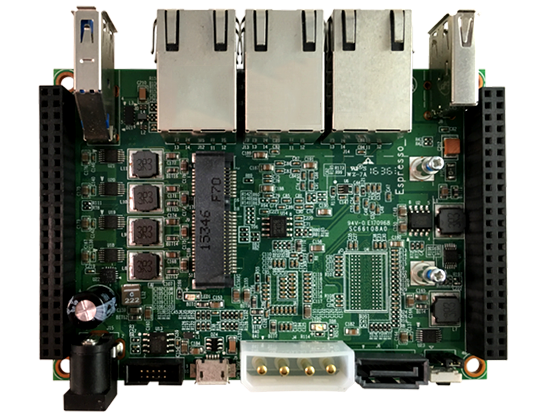
\includegraphics[width=5cm]{../slides/espressobin/espressobin.png}
  \end{center}
}


\def \training{buildroot}

% Title
\ifthenelse{\equal{\agendalanguage}{french}}{
  \def \trainingtitle{Formation développemment Linux embarqué avec Buildroot}
}{
  \def \trainingtitle{Embedded Linux development with Buildroot training}
}

% Duration
\ifthenelse{\equal{\trainingtype}{online}}{
  \def \trainingduration{5}
}{
  \def \trainingduration{3}
}

% Training objectives
\ifthenelse{\equal{\agendalanguage}{french}}{
  \def \traininggoals{
    \begin{itemize}
    \item Être capable de comprendre le principe d'un build system Linux
      embarqué, et comparer Buildroot aux autres outils offrant des
      fonctionnalités similaires.
    \item Être capable de créer un système Linux embarqué simple avec
      Buildroot: créer une configuration, lancer la compilation,
      installer le résultat sur une plateforme embarquée.
    \item Être capable d'ajuster la configuration de Buildroot pour
      construire un système Linux embarqué adapté à des besoins
      spécifiques: choix de la chaîne de compilation croisée, gestion de
      la configuration du noyau Linux, personnalisation du système de
      fichiers racine.
    \item Être capable de créer de nouveaux paquets dans Buildroot pour
      intégrer des applications et bibliothèques supplémentaires dans le
      système Linux embarqué.
    \item Être capable d'utiliser les outils proposés par Buildroot pour
      gérer et analyser le build: suivi des vulnérabilités, comformité
      aux licences open-source, etc.
    \item Être capable de développer et débugger des applications
      user-space Linux dans un contexte où Buildroot est utilisé.
    \item Être capable d'interagir avec la communauté open-source du
      projet Buildroot et de comprendre le fonctionnement interne de
      Buildroot.
    \end{itemize}
  }
}{
  \def \traininggoals{
    \begin{itemize}
    \item Be able to understand the role and principle of an embedded
      Linux build system, and compare Buildroot to other tools offering
      similar functionality.
    \item Be able to create a simple embedded Linux system with
      Buildroot: create a configuration, run the build, install the
      result on an embedded platform.
    \item Be able to adjust the Buildroot configuration to build an
      embedded Linux system tailored to specific needs: choice of the
      cross-compilation toolchain, management of the Linux kernel
      configuration, customization of the root filesystem contents, etc.
    \item Be able to create new packages in Buildroot to integrate
      additional applications and libraries into the embedded Linux
      system.
    \item Be able to use the tools offered by Buildroot to manage and
      analyze the build: security vulnerability tracking, license
      compliance, etc.
    \item Be able to develop and debug Linux user-space applications in
      the context of Buildroot.
    \item Be able to interact with the Buildroot open-source community,
      and to understand the internals of Buildroot.
    \end{itemize}
  }
}

% Training prerequisites
\def \trainingprerequisites{
  \begin{itemize}
    \prerequisitecommandline
    \prerequisiteembeddedlinux
    \prerequisiteenglish
  \end{itemize}
}

% Training audience
\ifthenelse{\equal{\agendalanguage}{french}}{
  \def \trainingaudience{
    Sociétés qui utilisent déjà Buildroot ou qui sont intéressées par
    l'utiliser pour construire leurs systèmes Linux embarqué.
  }
}{
  \def \trainingaudience{
    Companies already using or interested in using
    Buildroot to build their embedded Linux systems.
  }
}

% Time ratio
\def \onsitelecturetimeratio{40}
\def \onsitelabtimeratio{60}

% Agenda items

\defagendaitem
{intro}
{lecture}
{Embedded Linux and build system introduction}
{
  \begin{itemize}
  \item The general architecture of an embedded Linux system
  \item Build systems vs. binary distributions
  \item Role of a build system
  \item Comparison of existing build systems
  \end{itemize}
}
{Introduction à Buildroot et aux systèmes de build}
{
  \begin{itemize}
  \item Architecture générale d'une système Linux embarqué
  \item Choix entre systèmes de build et distributions binaires
  \item Rôle d'un système de build
  \item Comparaison des systèmes de build existants
  \end{itemize}
}
\defagendaitem
{introbuildroot}
{lecture}
{Introduction to Buildroot}
{
  \begin{itemize}
  \item Key facts about the project
  \item Getting Buildroot
  \item Basic configuration of Buildroot
  \item Doing a first build
  \end{itemize}
}
{Présentation de Buildroot}
{
  \begin{itemize}
  \item Points clés autour du projet
  \item Téléchargement des sources de Buildroot
  \item Configuration simple de Buildroot
  \item Exécution d'une premières compilation
  \end{itemize}
}
\defagendaitem
{basic}
{lab}
{Basic Buildroot usage}
{
  \begin{itemize}
  \item Getting and setting up Buildroot
  \item Configuring and building a basic system with Buildroot for an
    embedded platform
  \item Flash and test the generated system on the embedded platform
  \end{itemize}
}
{Utilisation simple de Buildroot}
{
  \begin{itemize}
  \item Téléchargement et configuration de Buildroot
  \item Configurer et compiler un système simple avec Buildroot pour
    un système embarqué
  \item Flasher et tester le système généré par Buildroot
  \end{itemize}
}
\defagendaitem
{configuration}
{lecture}
{Managing the build and configuration}
{
  \begin{itemize}
  \item Out of tree build
  \item Using and creating {\em defconfigs}
  \item Defconfig fragments
  \item Other building tips
  \end{itemize}
}
{Gestion de la compilation et de la configuration}
{
  \begin{itemize}
  \item Compilation en dehors des sources
  \item Utiliser et créer des fichiers {\em defconfigs}
  \item Fragments de {\em defconfigs}
  \item Autres astuces pour la compilation
  \end{itemize}
}
\defagendaitem
{buildrootsource}
{lecture}
{Buildroot source and build trees}
{
  \begin{itemize}
  \item Details about the Buildroot source code organization
  \item Details about the Buildroot build tree
  \end{itemize}
}
{Sources de Buildroot et arborescence des fichiers générés}
{
  \begin{itemize}
  \item Détails sur l'organisation du code source de Buildroot
  \item Détails sur l'arborescence des fichiers générés
  \end{itemize}
}
\defagendaitem
{toolchain}
{lecture}
{Toolchains in Buildroot}
{
  \begin{itemize}
  \item The different choices for using toolchains in Buildroot
  \item Overview of the toolchain options
  \item Using existing binary toolchains, such as Bootlin
    toolchains, understanding {\em multilib} capabilities and
    integration of toolchains in Buildroot
  \item Generating custom toolchains with {\em Crosstool-NG}, and
    re-use them as external toolchains
  \end{itemize}
}
{Chaînes de compilation {\em toolchains} dans Buildroot}
{
  \begin{itemize}
  \item Les différents possibilités d'usage de chaînes de compilation
	dans Buildroot.
  \item Tour d'horizon des options liées aux chaînes de compilation.
  \item Utilisation de chaînes des compilation binaires, comme
	celles de Bootlin. Détails sur les fonctionnalités
        {\em multilib} et l'intégration des toolchains dans Buildroot.
  \item Génération de toolchains sur mesure avec {\em Crosstool-NG},
	et leur utilisation comme chaînes externes.
  \end{itemize}
}
\defagendaitem
{manageconfiguration}
{lecture}
{Managing the Linux kernel configuration}
{
  \begin{itemize}
  \item Loading, changing and saving the kernel configuration
  \end{itemize}
}
{Gestion de la configuration du noyau Linux}
{
  \begin{itemize}
  \item Charger, modifier et sauvegarder la configuration du noyau.
  \end{itemize}
}
\defagendaitem
{rootfsconstruction}
{lecture}
{Root filesystem construction in Buildroot}
{
  \begin{itemize}
  \item Understand how Buildroot builds the root filesystem: {\em
      skeleton}, installation of packages, overlays, {\em post-build}
    and {\em post-image} scripts.
  \item Customization of the root filesystem contents
  \item System configuration: {\em console} selection, various {\tt
      /dev} management methods, the different {\tt init}
    implementations, etc.
  \item Understand how Buildroot generates filesystem images
  \end{itemize}
}
{Construction du système de fichier racine dans Buildroot}
{
  \begin{itemize}
  \item Comprendre comment Buildroot construit le système de fichiers
	racine : {\em skeleton}, installation de composants, {\em
        overlays}, scripts {\em post-build} et {\em post-image}.
  \item Personnalisation du contenu du système de fichiers
  \item Configuration du système : sélection de la {\em console},
	plusieurs méthode de gestion de {\tt /dev}, les différentes
	implémentations d'{\tt init}, etc.
  \item Comprendre comment Buildroot génère les images de systèmes de
	fichiers.
  \end{itemize}
}
\defagendaitem
{rootfscustomization}
{lab}
{Root filesystem customization}
{
  \begin{itemize}
  \item Explore the build output
  \item Customize the root filesystem using a {\em rootfs overlay}
  \item Customize the kernel with patches and additional configuration
    options
  \item Add more packages
  \item Use {\em defconfig} files and {\em out of tree} build
  \end{itemize}
}
{Personnalisation du système de fichiers}
{
  \begin{itemize}
  \item Exploration des fichiers générés
  \item Personnalisation du système de fichiers racine en utilisant un {\em rootfs overlay}
  \item Personnaliser le noyau avec des correctifs et des options de
	configuration supplémentaires
  \item Rajout de nouveaux composants
  \item Utilisation de fichiers {\em defconfig} et compilation en
	dehors des sources.
  \end{itemize}
}
\defagendaitem
{downloadbuildroot}
{lecture}
{Download infrastructure in Buildroot}
{
  \begin{itemize}
  \item Downloading logic
  \item Primary site and backup site, doing offline builds
  \item VCS download, integrity checking
  \item Download-related {\em make} targets
  \end{itemize}
}
{Infrastructure de téléchargement dans Buildroot}
{
  \begin{itemize}
  \item Méthodologie de téléchargement
  \item Site primaire et sites de backup, compilation en mode déconnecté
  \item Téléchargement via systèmes de contrôle de versions,
	vérification d'intégrité
  \item Cibles {\em make} en rapport avec les téléchargements
  \end{itemize}
}
\defagendaitem
{gnumake}
{lecture}
{GNU Make 101}
{
  \begin{itemize}
  \item Basics of make rules
  \item Defining and referencing variables
  \item Conditions, functions
  \item Writing recipes
  \end{itemize}
}
{Introduction à GNU Make}
{
  \begin{itemize}
  \item Éléments de base des règles de make
  \item Définition et utilisation de variables
  \item Conditions et fonctions
  \item Écriture de recettes
  \end{itemize}
}
\defagendaitem
{newpackage}
{lecture}
{Integrating new packages in Buildroot}
{
  \begin{itemize}
  \item How to integrate new packages in the Buildroot configuration
    system
  \item Understand the different package infrastructures: for {\em
      generic}, {\em autotools}, {\em CMake}, {\em Python} packages
    and more.
  \item Writing a package \code{Config.in} file: how to express
    dependencies on other packages, on toolchain options, etc.
  \item Details on writing a package recipe: describing the package
    source code location, download method, configuration, build and
    installation steps, handling dependencies, etc.
  \end{itemize}
}
{Intégration de nouveaux composants dans Buildroot}
{
  \begin{itemize}
  \item Comment rajouter de nouveaux paquetages au système de
	configuration de Buildroot
  \item Comprendre les différentes infrastructures de paquetages : pour
	des composants {\em generic}, {\em autotools}, {\em CMake}, {\em
	Python} et autres
  \item Écriture un fichier \code{Config.in} pour un composant : comment
    exprimer des dépendances vers d'autres composants, vers des options
    de toolchains, etc.
  \item Détails sur l'écriture d'une recette pour un composant :
	description de l'emplacement du code source, de la méthode de
	téléchargement, de configuration, de compilation et
	d'installation, gestion des dépendances, etc. 
  \end{itemize}
}
\defagendaitem
{newpackage}
{lab}
{New packages in Buildroot}
{
  \begin{itemize}
  \item Create a new package for {\em nInvaders}
  \item Understand how to add dependencies
  \item Add patches to {\em nInvaders} for {\em Nunchuk} support
  \end{itemize}
}
{Nouveaux composants dans Buildroot}
{
  \begin{itemize}
  \item Création d'un nouveau paquetage pour {\em nInvaders}
  \item Comprendre comment rajouter des dépendances
  \item Ajouter des correctifs pour {\em nInvaders} pour prendre en
	charge le contrôle via un {\em Nunchuk}
  \end{itemize}
}
\defagendaitem
{advancepackage}
{lecture}
{Advanced package aspects}
{
  \begin{itemize}
  \item Licensing report
  \item Patching support: patch ordering and format, global patch directory, etc.
  \item User, permission, device tables
  \item Init scripts and systemd unit files
  \item Config scripts
  \item Understanding {\em hooks}
  \item Overriding commands
  \item Legacy handling
  \item Virtual packages
  \end{itemize}
}
{Notions avancées sur les paquetages}
{
  \begin{itemize}
  \item Rapport de licences
  \item Prise en charge des correctifs : ordre d'application et format,
	répertoire global pour les correctifs, etc.
  \item Utilisateur, droit d'accès, tables de fichiers devices
  \item Script d'init et fichiers unitaires pour systemd
  \item Scripts de configuration
  \item Compréhension des {\em hooks}
  \item Surcharger des commandes
  \item Gestion des paquetages legacy
  \item Paquetages virtuels
  \end{itemize}
}
\defagendaitem
{advancepackage}
{lab}
{Advanced packages}
{
  \begin{itemize}
  \item Package an application with a mandatory dependency and an
    optional dependency
  \item Package a library, hosted on GitHub
  \item Use {\em hooks} to tweak packages
  \item Add a patch to a package
  \end{itemize}
}
{Paquetages avancés}
{
  \begin{itemize}
  \item Packager une application avec une dépendance obligatoire et
    une dépendance optionnelle
  \item Packager une bibliothèque, hébergée sur GitHub
  \item Utilisation de {\em hooks} pour ajuster les paquetages
  \item Rajouter un correctif à un paquetage
  \end{itemize}
}
\defagendaitem
{analyzebuild}
{lecture}
{Analyzing the build: licensing, dependencies, build time}
{
  \begin{itemize}
  \item Usage of the legal information infrastructure
  \item Graphing dependencies of packages
  \item Collecting and graphing build time information
  \end{itemize}
}
{Analyse d'une compilation : licences, dépendances, temps de
construction}
{
  \begin{itemize}
  \item Utilisation de l'infrastructure de gestion des informations
	légales
  \item Représentation graphique des dépendances entre paquetages
  \item Collecte d'informations et représentation du temps de
	compilation
  \end{itemize}
}
\defagendaitem
{advanced}
{lecture}
{Advanced topics}
{
  \begin{itemize}
  \item \code{BR2_EXTERNAL} to store customizations outside of the
    Buildroot sources
  \item Package-specific targets
  \item Understanding rebuilds
  \item Tips for building faster
  \end{itemize}
}
{Sujets avancés}
{
  \begin{itemize}
  \item \code{BR2_EXTERNAL} pour stocker des personnalisations à
	l'extérieur des sources de Buildroot
  \item Cibles make spécifiques pour les paquetages
  \item Comprendre les recompilations
  \item Astuces pour compiler plus vite
  \end{itemize}
}
\defagendaitem
{advanced}
{lab}
{Advanced aspects}
{
  \begin{itemize}
  \item Use build time graphing capabilities
  \item Use dependency graphing capabilities
  \item Use licensing report generation, and add licensing
    information to your own packages
  \item Use \code{BR2_EXTERNAL}
  \end{itemize}
}
{Sujets avancés}
{
  \begin{itemize}
  \item Utilisation des capacités de génération de graphes de temps de
	compilation
  \item Génération de graphes de dépendances
  \item Utilisation du rapport sur les licences, et ajout d'informations
	légales à vos propres paquetages 
  \item Utilisation de \code{BR2_EXTERNAL}
  \end{itemize}
}
\defagendaitem
{appdevelopment}
{lecture}
{Application development with Buildroot}
{
  \begin{itemize}
  \item Using Buildroot during application development
  \item Usage of the Buildroot environment to build applications
    outside of Buildroot
  \item Generate an SDK for other developers
  \item Remote debugging with Buildroot
  \end{itemize}
}
{Développement applicatif avec Buildroot}
{
  \begin{itemize}
  \item Utilisation de Buildroot pendant le développement d'applications
  \item Utilisation de l'environnement de Buildroot pour compiler des
	applications en dehors de Buildroot
  \item Générer un SDK pour d'autres développeurs
  \item Débug à distance avec Buildroot
  \end{itemize}
}
\defagendaitem
{appdevelopment}
{lab}
{Application development with Buildroot}
{
  \begin{itemize}
  \item Build and run your own application
  \item Remote debug your application
  \item Use \code{<pkg>_OVERRIDE_SRCDIR}
  \end{itemize}
}
{Développement applicatif avec Buildroot}
{
  \begin{itemize}
  \item Compiler et exécuter votre propre application
  \item Débug à distance de votre application
  \item Utilisation de \code{<pkg>_OVERRIDE_SRCDIR}
  \end{itemize}
}
\defagendaitem
{internals}
{lecture}
{Understanding Buildroot internals}
{
  \begin{itemize}
  \item Detailed description of the Buildroot build process:
    toolchain, packages, root filesystem construction, stamp files,
    etc.
  \item Understanding virtual packages.
  \end{itemize}
}
{Comprendre les mécanismes internes de Buildroot}
{
  \begin{itemize}
  \item Description détaillée du processus de compilation de Buildroot :
    	toolchain, paquetages, construction du système de fichiers race,
	fichiers {\em stamp}, etc.
  \item Comprendre les paquetages virtuels.
  \end{itemize}
}
\defagendaitem
{support}
{lecture}
{Getting support and contributing}
{
  \begin{itemize}
  \item Getting support: {\em Bugzilla}, {\em mailing list}, {\em IRC}
  \item Contributing: understanding the development process, how to
    submit patches
  \end{itemize}
}
{Obtenir de l'aide et s'impliquer}
{
  \begin{itemize}
  \item Obtenir de l'assistance technique : {\em Bugzilla}, {\em liste de
	discussion}, {\em IRC}
  \item Contribuer : comprendre le processus de développement, comment
    soumettre des correctifs
  \end{itemize}
}

\def \onlineagenda {
  \showonlineagendaday{1}
  \showagendaitem{intro}{lecture}
  \showagendaitem{introbuildroot}{lecture}
  \showagendaitem{basic}{lab}
  \showagendaitem{configuration}{lecture}
  \showagendaitem{buildrootsource}{lecture}
  \showonlineagendaday{2}
  \showagendaitem{toolchain}{lecture}
  \showagendaitem{manageconfiguration}{lecture}
  \showagendaitem{rootfsconstruction}{lecture}
  \showagendaitem{rootfscustomization}{lab}
  \showagendaitem{downloadbuildroot}{lecture}
  \showonlineagendaday{3}
  \showagendaitem{gnumake}{lecture}
  \showagendaitem{newpackage}{lecture}
  \showagendaitem{newpackage}{lab}
  \showagendaitem{advancepackage}{lecture}
  \showonlineagendaday{4}
  \showagendaitem{advancepackage}{lab}
  \showagendaitem{analyzebuild}{lecture}
  \showagendaitem{advanced}{lecture}
  \showagendaitem{advanced}{lab}
  \showonlineagendaday{5}
  \showagendaitem{appdevelopment}{lecture}
  \showagendaitem{appdevelopment}{lab}
  \showagendaitem{internals}{lecture}
  \showagendaitem{support}{lecture}
  \showagendaitem{qna}{misc}
}

\def \onsiteagenda {
  \showonlineagendaday{1}
  \showagendaitem{intro}{lecture}
  \showagendaitem{introbuildroot}{lecture}
  \showagendaitem{basic}{lab}
  \showagendaitem{configuration}{lecture}
  \showonlineagendaday{2}
  \showagendaitem{buildrootsource}{lecture}
  \showagendaitem{toolchain}{lecture}
  \showagendaitem{manageconfiguration}{lecture}
  \showagendaitem{rootfsconstruction}{lecture}
  \showagendaitem{rootfscustomization}{lab}
  \showonlineagendaday{3}
  \showagendaitem{downloadbuildroot}{lecture}
  \showagendaitem{gnumake}{lecture}
  \showagendaitem{newpackage}{lecture}
  \showagendaitem{newpackage}{lab}
  \showonlineagendaday{4}
  \showagendaitem{advancepackage}{lecture}
  \showagendaitem{advancepackage}{lab}
  \showonlineagendaday{5}
  \showagendaitem{analyzebuild}{lecture}
  \showagendaitem{advanced}{lecture}
  \showagendaitem{advanced}{lab}
  \showonlineagendaday{6}
  \showagendaitem{appdevelopment}{lecture}
  \showagendaitem{appdevelopment}{lab}
  \showagendaitem{internals}{lecture}
  \showagendaitem{support}{lecture}
}
